\documentclass{beamer}
\usepackage[utf8]{inputenc}
\usepackage{tikz}
\usetikzlibrary{positioning}
\usetheme{Madrid}
\usepackage{listings}
\usepackage{booktabs}
\usepackage[backend=biber,style=authoryear-comp]{biblatex}
\usecolortheme{default}
\usepackage{caption}
\usepackage{subcaption}
\usepackage{tcolorbox}
\usepackage{svg}
\usepackage{xcolor}
\usepackage{algorithm2e}
\usepackage{fourier}
\newtheorem{proposition}{Proposition}
\setbeamertemplate{navigation symbols}{}
% Code styling
\definecolor{codegreen}{rgb}{0,0.6,0}
\definecolor{codegray}{rgb}{0.5,0.5,0.5}
\definecolor{codepurple}{rgb}{0.58,0,0.82}
\definecolor{backcolour}{rgb}{0.95,0.95,0.92}

\lstdefinestyle{mystyle}{
    backgroundcolor=\color{backcolour},   
    commentstyle=\color{codegreen},
    keywordstyle=\color{magenta},
    numberstyle=\color{codegray},
    stringstyle=\color{codepurple},
    basicstyle=\ttfamily\tiny,
    breakatwhitespace=false,         
    breaklines=True,                 
    captionpos=b,                    
    keepspaces=true,                 
    numbers=none,                    
    showspaces=false,                
    showstringspaces=false,
    showtabs=false,                  
    tabsize=2
}

\lstset{style=mystyle}
%------------------------------------------------------------
%This block of code defines the information to appear in the
%Title page
\addbibresource{bibliographie.bib}
\title %optional
[Interpretable RL]{Interpretability, Decision Trees, and Sequential Decision Making}

\author[Hector Kohler] % (optional)
{Hector Kohler}

\institute[Univ. Lille] % (optional)
{
  Supervised by Dr. Riad Akrour (HdR) and Prof. Philippe Preux (HdR)\\
  Universit\'e de Lille, CNRS, Inria, UMR CRIStAL 9189, France
}

\begin{document}

\frame{\titlepage}


%% -----------------------INTRO-----------------------
\begin{frame}{Sequential decision making (SDM)}
\begin{figure}
    \centering
    \begin{tikzpicture}[
        node distance=2.5cm,
        auto,
        thick,
        state/.style={circle, draw, fill=blue!20, minimum size=1.5cm, text centered},
        environment/.style={rectangle, draw, dashed, fill=blue!10, rounded corners, minimum width=4cm, minimum height=2cm, text centered},
        ml/.style={circle, draw, fill=purple!20, minimum width=1cm, minimum height=1cm, text centered},
        agent/.style={rectangle, draw, fill=orange!20, rounded corners, minimum width=2cm, minimum height=1.5cm, text centered},
        nn/.style={rectangle, draw, fill=black!20, rounded corners, minimum width=2cm, minimum height=1.5cm, text centered},
        robot/.style={rectangle, draw, fill=green!20, rounded corners, minimum width=2cm, minimum height=1.5cm, text centered},
        decision_box/.style={rectangle, draw, dashed, fill=gray!10, minimum width=5cm, minimum height=2.7cm, text centered},
        big_decision_box/.style={rectangle, draw, dashed, fill=gray!10, minimum width=7cm, minimum height=2.7cm, text centered},
        arrow/.style={->, thick, bend left=15},
        arrow_decision/.style={->, dashed, bend left=15},
        ml/.style={circle, draw, fill=purple!20, minimum width=1cm, minimum height=1cm, text centered},
    ]
        
        % Decision Making Box
        \node<1>[decision_box] (decision_box) at (0,3.8) {};
        \node<2->[big_decision_box] (big_decision_box) at (0,3.8) {};
        \node at (0,4.7) {\textbf{Decision Making}};
        
        % %Robot (AI)
        % \node<2>[robot] (robot) at (-4.1,3.4) {
        %     \begin{minipage}{1.5cm}
        %         \centering
        %         \includesvg[width=0.4cm]{../images/images_intro/robot-svgrepo-com.svg}\\
        %         \small{Policy}
        %     \end{minipage}
        % };
        % \node<5->[ml] (ml) at (-6,3) {
        %     \begin{minipage}{1cm}
        %         \centering
        %         \includesvg[width=0.4cm]{../images/images_intro/gear-file-svgrepo-com.svg}\\
        %         \small{ML}
        %     \end{minipage}
        % };
        \node<2->[robot] (robot_) at (-2.1,3.4) {
            \begin{minipage}{1.5cm}
                \centering
                \includesvg[width=0.4cm]{../images/images_intro/robot-svgrepo-com.svg}\\
                \small{Policy}
            \end{minipage}
        };
        
        % Doctor
        \node<1>[agent] (doctor) at (0,3.4) {
            \begin{minipage}{1.5cm}
                \centering
                \includesvg[width=0.4cm]{../images/images_intro/doctor-with-stethoscope-svgrepo-com.svg}\\
                \small{Doctor}
            \end{minipage}
        };

        \node<2>[agent] (doctor_) at (2.1,3.4) {
            \begin{minipage}{1.5cm}
                \centering
                \includesvg[width=0.4cm]{../images/images_intro/doctor-with-stethoscope-svgrepo-com.svg}\\
                \small{Doctor}
            \end{minipage}
        };

        % \node<8->[nn] (nn_) at (-2.1,3.4) {
        %     \begin{minipage}{1.5cm}
        %         \centering
        %         \includesvg[width=0.4cm]{../images/images_intro/network-mapping-svgrepo-com.svg}\\
        %         \small{Neural network}
        %     \end{minipage}
        % };
        
        % Environment (Patient)
        \node[environment] (environment) at (0,-0.5) {
            \begin{minipage}{2cm}
                \centering
                \includesvg[width=0.8cm]{../images/images_intro/patient-4.svg}\\
                \small{Cancer patient}
            \end{minipage}
        };
        
        % Arrows
        \draw<1>[arrow] (environment) to[bend left=30] node[left] {
            \begin{minipage}{2cm}
                \centering
                \includesvg[width=0.4cm]{../images/images_intro/patient-clipboard-svgrepo-com.svg}\\
                \small{Updated health status}
            \end{minipage}
        } (doctor);
        \draw<2->[arrow] (environment) to[bend left=30] node[left] {
            \begin{minipage}{2cm}
                \centering
                \includesvg[width=0.4cm]{../images/images_intro/patient-clipboard-svgrepo-com.svg}\\
                \small{Updated health status}
            \end{minipage}
        } (robot_);
        % \draw<8->[arrow] (environment) to[bend left=30] node[left] {
        %     \begin{minipage}{2cm}
        %         \centering
        %         \includesvg[width=0.4cm]{../images/images_intro/patient-clipboard-svgrepo-com.svg}\\
        %         \small{Updated health status}
        %     \end{minipage}
        % } (nn_);
        \draw<2->[arrow_decision] (robot_) to node[above] {\small{Recommends}} (doctor_);
        % \draw<8->[arrow_decision] (nn_) to node[above] {\small{Recommends}} (doctor_);
        % \draw<4-7>[arrow_decision] (doctor_) to node[below] {\small{Interprets}} (robot_);
        % \draw<8->[arrow_decision, red] (doctor_) to node[below] {\small{Cannot interpret}} (nn_);

        \draw<1>[arrow] (doctor) to[bend left=30] node[right] {
            \begin{minipage}{3cm}
                \centering
                \includesvg[width=0.5cm]{../images/images_intro/syringe-svgrepo-com.svg}\\
                \small{Administers chemotherapy}
            \end{minipage}
        } (environment);
        \draw<2->[arrow] (doctor_) to[bend left=30] node[right] {
            \begin{minipage}{3cm}
                \centering
                \includesvg[width=0.5cm]{../images/images_intro/syringe-svgrepo-com.svg}\\
                \small{Administers chemotherapy}
            \end{minipage}
        } (environment);
        % ML learning arrows
        % \draw<6->[arrow] (environment) to[bend left=40] node[left] {
        %     \begin{minipage}{2cm}
        %         \centering
        %         \includesvg[width=0.5cm]{../images/images_intro/patient-clipboard-svgrepo-com.svg}\\
        %         \small{Treatment outcomes}
        %     \end{minipage}
        % } (ml);
        % \draw<7>[arrow] (ml) to[bend left=20] node[above] {
        %     \begin{minipage}{1.5cm}
        %         \centering
        %         \small{Updates}
        %     \end{minipage}
        % } (robot_);
        % \draw<8->[arrow] (ml) to[bend left=20] node[above] {
        %     \begin{minipage}{1.5cm}
        %         \centering
        %         \small{Updates}
        %     \end{minipage}
        % } (nn_);

        
        
    \end{tikzpicture}
\end{figure}
\end{frame}


\begin{frame}{Markov decision processes (MDPs) and reinforcement learning (RL)}
\begin{minipage}{0.53\textwidth}
    \begin{figure}
        \centering
        \scalebox{0.85}{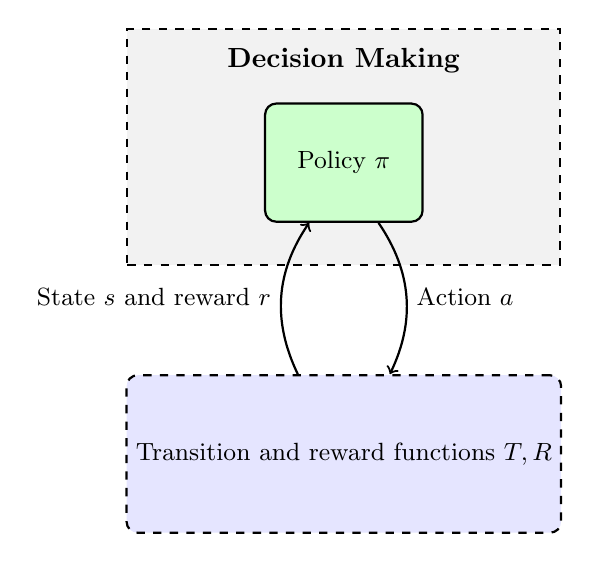
\begin{tikzpicture}[
            node distance=2.5cm,
            auto,
            thick,
            state/.style={circle, draw, fill=blue!20, minimum size=1.5cm, text centered},
            environment/.style={rectangle, draw, dashed, fill=blue!10, rounded corners, minimum width=4cm, minimum height=2cm, text centered},
            agent/.style={rectangle, draw, fill=orange!20, rounded corners, minimum width=2cm, minimum height=1.5cm, text centered},
            robot/.style={rectangle, draw, fill=green!20, rounded corners, minimum width=2cm, minimum height=1.5cm, text centered},
            decision_box/.style={rectangle, draw, dashed, fill=gray!10, minimum width=5.5cm, minimum height=3cm, text centered},
            arrow/.style={->, thick, bend left=15},
            arrow_decision/.style={->, dashed, bend left=15}
        ]
            
            % Decision Making Box
            \node[decision_box] (decision_box) at (0,3.4) {};
            \node at (0,4.5) {\textbf{Decision Making}};
            
            % Robot (AI)
            \node[robot] (robot) at (0,3.2) {\small{Policy $\pi$}};
            
            
            % Environment (Patient)
            \node[environment] (environment) at (0,-0.5) {\small{Transition and reward functions $T, R$}};
            
            % Arrows
            \draw[arrow] (environment) to[bend left=30] node[left] {\small{State $\boldsymbol{s}$ and reward $r$}} (robot);
            \draw[arrow] (robot) to[bend left=30] node[right] {\small{Action $a$}} (environment);
            
        \end{tikzpicture}}
        \caption*{Markov decision processes {\small \textcolor{purple}{\parencite{puterman}}}.}
    \end{figure}
\end{minipage}%
\begin{minipage}{0.46\textwidth}
    \begin{itemize}
        \item<2-> RL {\small \textcolor{purple}{\small \parencite{sutton}}} aims to find a policy, $\pi: S \rightarrow A$ that maximizes:
        \[J(\pi) = \underset{\boldsymbol{s}_{t}\sim T}{\mathbb{E}}\left[\sum_{t=0}^{\infty} \gamma^t R(s_t, \pi(s_t))\right]\]
        
        \item<3-> Lots of succesful (deep) RL algorithms {\small \textcolor{purple}{\parencite{ppo}}}.
        % \item<4-> Few interpretability concerns.
    \end{itemize}
\end{minipage}
\end{frame}

\begin{frame}{Sequential decision making (SDM) and machine learning (ML)}
\begin{figure}
    \centering
    \begin{tikzpicture}[
        node distance=2.5cm,
        auto,
        thick,
        state/.style={circle, draw, fill=blue!20, minimum size=1.5cm, text centered},
        environment/.style={rectangle, draw, dashed, fill=blue!10, rounded corners, minimum width=4cm, minimum height=2cm, text centered},
        ml/.style={circle, draw, fill=purple!20, minimum width=1cm, minimum height=1cm, text centered},
        agent/.style={rectangle, draw, fill=orange!20, rounded corners, minimum width=2cm, minimum height=1.5cm, text centered},
        nn/.style={rectangle, draw, fill=black!20, rounded corners, minimum width=2cm, minimum height=1.5cm, text centered},
        robot/.style={rectangle, draw, fill=green!20, rounded corners, minimum width=2cm, minimum height=1.5cm, text centered},
        decision_box/.style={rectangle, draw, dashed, fill=gray!10, minimum width=5cm, minimum height=2.7cm, text centered},
        big_decision_box/.style={rectangle, draw, dashed, fill=gray!10, minimum width=7cm, minimum height=2.7cm, text centered},
        arrow/.style={->, thick, bend left=15},
        arrow_decision/.style={->, dashed, bend left=15},
        ml/.style={circle, draw, fill=purple!20, minimum width=1cm, minimum height=1cm, text centered},
    ]
        
        % Decision Making Box
        \node[decision_box] (decision_box) at (0,3.8) {};
        \node[big_decision_box] (big_decision_box) at (0,3.8) {};
        \node at (0,4.7) {\textbf{Decision Making}};
        
        % %Robot (AI)
        % \node[robot] (robot) at (-4.1,3.4) {
        %     \begin{minipage}{1.5cm}
        %         \centering
        %         \includesvg[width=0.4cm]{../images/images_intro/robot-svgrepo-com.svg}\\
        %         \small{Policy}
        %     \end{minipage}
        % };
        \node<1->[ml] (ml) at (-6,3) {
            \begin{minipage}{1cm}
                \centering
                \includesvg[width=0.4cm]{../images/images_intro/gear-file-svgrepo-com.svg}\\
                \small{RL}
            \end{minipage}
        };
        \node<1>[robot] (robot_) at (-2.1,3.4) {
            \begin{minipage}{1.5cm}
                \centering
                \includesvg[width=0.4cm]{../images/images_intro/robot-svgrepo-com.svg}\\
                \small{Policy}
            \end{minipage}
        };
        
        % Doctor
        % \node<1-2>[agent] (doctor) at (0,3.4) {
        %     \begin{minipage}{1.5cm}
        %         \centering
        %         \includesvg[width=0.4cm]{../images/images_intro/doctor-with-stethoscope-svgrepo-com.svg}\\
        %         \small{Doctor}
        %     \end{minipage}
        % };

        \node[agent] (doctor_) at (2.1,3.4) {
            \begin{minipage}{1.5cm}
                \centering
                \includesvg[width=0.4cm]{../images/images_intro/doctor-with-stethoscope-svgrepo-com.svg}\\
                \small{Doctor}
            \end{minipage}
        };

        \node<2->[nn] (nn_) at (-2.1,3.4) {
            \begin{minipage}{1.5cm}
                \centering
                \includesvg[width=0.4cm]{../images/images_intro/network-mapping-svgrepo-com.svg}\\
                \small{Neural network}
            \end{minipage}
        };
        
        % Environment (Patient)
        \node[environment] (environment) at (0,-0.5) {
            \begin{minipage}{2cm}
                \centering
                \includesvg[width=0.8cm]{../images/images_intro/patient-4.svg}\\
                \small{Cancer patient}
            \end{minipage}
        };
        
        % Arrows
        
        \draw<1>[arrow] (environment) to[bend left=30] node[left] {
            \begin{minipage}{2cm}
                \centering
                \includesvg[width=0.4cm]{../images/images_intro/patient-clipboard-svgrepo-com.svg}\\
                \small{Updated health status}
            \end{minipage}
        } (robot_);
        \draw<2->[arrow] (environment) to[bend left=30] node[left] {
            \begin{minipage}{2cm}
                \centering
                \includesvg[width=0.4cm]{../images/images_intro/patient-clipboard-svgrepo-com.svg}\\
                \small{Updated health status}
            \end{minipage}
        } (nn_);
        \draw<1>[arrow_decision] (robot_) to node[above] {\small{Recommends}} (doctor_);
        \draw<2->[arrow_decision] (nn_) to node[above] {\small{Recommends}} (doctor_);
        % \draw<1-3>[arrow_decision] (doctor_) to node[below] {\small{Interprets}} (robot_);
        \draw<3->[arrow_decision, red] (doctor_) to node[below] {\small{Cannot interpret}} (nn_);

        % \draw<1-2>[arrow] (doctor) to[bend left=30] node[right] {
        %     \begin{minipage}{3cm}
        %         \centering
        %         \includesvg[width=0.5cm]{../images/images_intro/syringe-svgrepo-com.svg}\\
        %         \small{Administers chemotherapy}
        %     \end{minipage}
        % } (environment);
        \draw<1->[arrow] (doctor_) to[bend left=30] node[right] {
            \begin{minipage}{3cm}
                \centering
                \includesvg[width=0.5cm]{../images/images_intro/syringe-svgrepo-com.svg}\\
                \small{Administers chemotherapy}
            \end{minipage}
        } (environment);
        % ML learning arrows
        \draw<1->[arrow] (environment) to[bend left=40] node[left] {
            \begin{minipage}{2cm}
                \centering
                \includesvg[width=0.5cm]{../images/images_intro/patient-clipboard-svgrepo-com.svg}\\
                \small{}
            \end{minipage}
        } (ml);


        \draw<1>[arrow] (ml) to[bend left=20] node[above] {
            \begin{minipage}{1.5cm}
                \centering
                \small{Updates}
            \end{minipage}
        } (robot_);

        \draw<2->[arrow] (ml) to[bend left=20] node[above] {
            \begin{minipage}{1.5cm}
                \centering
                \small{Updates}
            \end{minipage}
        } (nn_);

        
        
    \end{tikzpicture}
\end{figure}
\end{frame}

\begin{frame}{Interpretability in SDM {\small \parencite{glanois-survey}}.}
    \only<1>{\textbf{\warning No concensus on definition \textcolor{purple}{\small \parencite{lipton}}}.}
    \only<2>{\begin{figure}
        \begin{subfigure}{0.45\textwidth}
        \centering
        \includegraphics[width=0.95\textwidth]{../images/images_intro/breakout_reflect_bp.png}
        \end{subfigure}
        \hfill
        \begin{subfigure}{0.45\textwidth}
        \centering
        \includegraphics[width=0.95\textwidth]{../images/images_intro/breakout_reflect.png}
        \end{subfigure}
        \caption*{Saliency maps of different MDP states \textcolor{purple}{\small \parencite{saliency}}.}
    \end{figure}}
    % \only<3>{
    %     \begin{figure}
    %         \centering
    %         \includegraphics[width=0.9\textwidth]{../images/lime.png}
    %         \caption*{Local interpretable model-agnostic explanations (LIME) \textcolor{purple}{\small \parencite{lime}}.}
    %     \end{figure}
    % }
    \only<3->{
        \begin{figure}
    \centering
    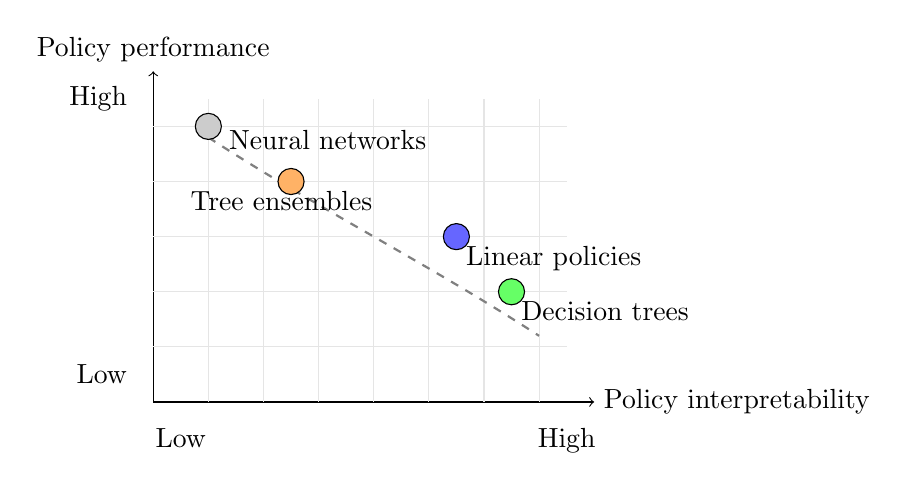
\begin{tikzpicture}[scale=0.7]
        % Define the axes
        \draw[->] (0,0) -- (8,0) node[right] {Policy interpretability};
        \draw[->] (0,0) -- (0,6) node[above] {Policy performance};
        
        % Add axis labels at the ends
        \node[below] at (0.5,-0.3) {Low};
        \node[below] at (7.5,-0.3) {High};
        \node[left] at (-0.3,0.5) {Low};
        \node[left] at (-0.3,5.5) {High};
        
        % Add grid lines (optional, subtle)
        \foreach \x in {1,2,...,7}
            \draw[gray!20] (\x,0) -- (\x,5.5);
        \foreach \y in {1,2,...,5}
            \draw[gray!20] (0,\y) -- (7.5,\y);
        
        % Add a general trend line (optional)
        \draw[dashed, thick, gray] (1,4.8) .. controls (3,3.5) and (5,2.5) .. (7,1.2);
        
        % Position different model types
        % Deep Neural Networks (high performance, low interpretability)
        \node[circle, fill=black!20, draw, minimum size=8pt] at (1,5) {};
        \node[below right] at (1.2,5.1) {Neural networks};
        
        % Ensemble Methods (medium-high performance, low-medium interpretability)
        \node[circle, fill=orange!60, draw, minimum size=8pt] at (2.5,4) {};
        \node[below right] at (0.5,4) {Tree ensembles};
        
        % Linear Models (medium performance, high interpretability)
        \node[circle, fill=blue!60, draw, minimum size=8pt] at (5.5,3) {};
        \node[below right] at (5.5,3) {Linear policies};
        
        % Decision Trees (medium-low performance, high interpretability)
        \node[circle, fill=green!60, draw, minimum size=8pt] at (6.5,2) {};
        \node[below right] at (6.5,2) {Decision trees};
        
    \end{tikzpicture}
    \only<3>{\caption*{Global interpretation.}}
\end{figure}
    }
\end{frame}

\begin{frame}{Decision trees}
\begin{figure}
    \centering
    \scalebox{0.8}{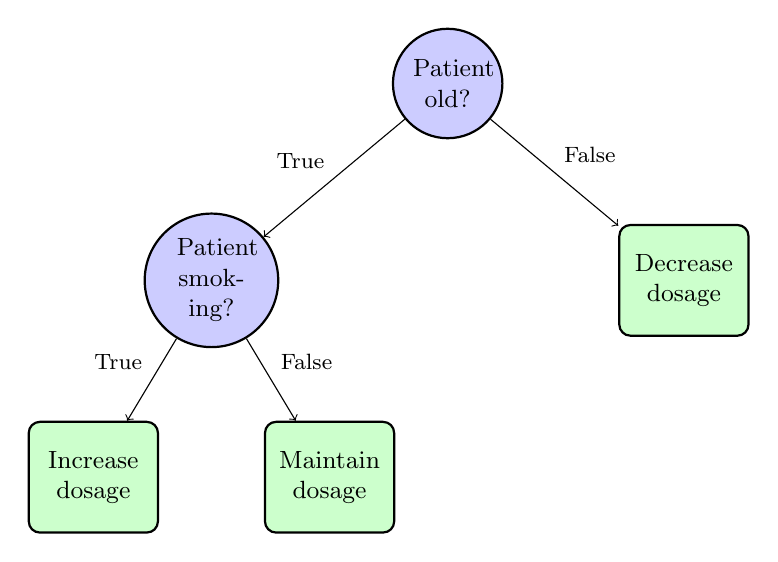
\begin{tikzpicture}[
        scale=1.0,
        decision/.style={circle, draw, thick, fill=blue!20, text width=2.5em, text centered, minimum height=2.5em, font=\small},
        leaf/.style={rectangle, draw, thick, fill=green!20, text width=4em, text centered, rounded corners, minimum height=4em, font=\small},
        edge_label/.style={font=\footnotesize, midway}
    ]
        % Root decision node
        \node[decision] (root) at (0,0) {Patient old?};
        
        % Second level nodes
        \node[decision] (left_decision) at (-3, -2.5) {Patient smoking?};
        \node[leaf] (right_leaf) at (3, -2.5) {Decrease dosage};
        
        % Third level nodes (leaves)
        \node[leaf] (left_left) at (-4.5, -5) {Increase dosage};
        \node[leaf] (left_right) at (-1.5, -5) {Maintain dosage};
        
        % Connections with labels
        \draw[->] (root) -- (left_decision) node[edge_label, above left] {True};
        \draw[->] (root) -- (right_leaf) node[edge_label, above right] {False};
        \draw[->] (left_decision) -- (left_left) node[edge_label, above left] {True};
        \draw[->] (left_decision) -- (left_right) node[edge_label, above right] {False};
        
        % Add labels for components
        % \node[font=\footnotesize, text=gray] at (0, 0.8) {Root node with test $t_1(x_i)$};
        % \node[font=\footnotesize, text=gray] at (-6, -2.5) {Internal node with test $t_2(x_i)$};
        % \node[font=\footnotesize, text=gray] at (-3, -5.8) {Leaf nodes with predictions};
        
    \end{tikzpicture}}
    \caption*{A generic decision tree of depth $D=2$.}
\end{figure}
\pause
Successful algorithms for classification/regression {\small \textcolor{purple}{\parencite{breiman1984classification}}}.
\\
\pause
\textbf{\textcolor{blue}{What about SDM?}}
\end{frame}

\begin{frame}{Imitation learning}
\begin{figure}
    \centering
    \includegraphics[width=1\textwidth]{Capture d’écran du 2023-09-04 14-56-36.png}
\end{figure}
\onslide<2->{Most research focused on indirect learning of interpretable policies {\small \textcolor{purple}{\parencite{viper}}}.}\\
\end{frame}

\begin{frame}{Two ways to get interpretable policies for SDM {\small \parencite{glanois-survey}}}
\begin{figure}
    \centering
    \scalebox{0.82}{
    \begin{tikzpicture}[
        node distance=2cm,
        scale=1,
        auto,
        thick,
        rl/.style={circle, draw, fill=purple!20, minimum width=1.5cm, minimum height=0.8cm, text centered},
        nn/.style={rectangle, draw, fill=black!20, rounded corners, minimum width=1.5cm, minimum height=1cm, text centered},
        sl/.style={circle, draw, fill=blue!20, minimum width=1.5cm, minimum height=0.8cm, text centered},
        dt/.style={rectangle, draw, fill=green!20, rounded corners, minimum width=1.5cm, minimum height=1cm, text centered},
        arrow/.style={->, thick},
        label/.style={font=\tiny, above},
        method_box/.style={rectangle, draw, dashed, minimum width=5cm, minimum height=3cm, text centered},
        method_box_indirect/.style={rectangle, draw, dashed, minimum width=9.5cm, minimum height=3cm, text centered}
    ]
        
        % Direct method box
        \node<3->[method_box] (direct_box) at (-0.5,0) {};
        \node<3-> at (-0.5,1.7) {\small{\textcolor{blue}{\textbf{Direct?}}}};
        
        % Direct method - RL process
        \node<4->[rl] (rl_direct) at (-2,0) {
            \begin{minipage}{1.2cm}
                \centering
                \includesvg[width=0.3cm]{../images/images_intro/gear-file-svgrepo-com.svg}\\
                \tiny{Reinforcement learning}
            \end{minipage}
        };
        
        % Direct method - Decision Tree
        \node<4->[dt] (dt_direct) at (1,0) {
            \begin{minipage}{1.2cm}
                \centering
                \includesvg[width=0.3cm]{../images/images_intro/decision-tree-svgrepo-com.svg}\\
                \tiny{Decision tree}
            \end{minipage}
        };
        
        % Direct method arrow
        \draw<4->[arrow] (rl_direct) -- (dt_direct) node[label, midway] {\tiny Learns};
        
        % Indirect method box
        \node<1->[method_box_indirect] (indirect_box) at (7.1,0) {};
        \node<1-> at (6.8,1.7) {\small{Indirect}};
        
        % Indirect method - RL process
        \node<1->[rl] (rl_indirect) at (3.5,0) {
            \begin{minipage}{1.2cm}
                \centering
                \includesvg[width=0.3cm]{../images/images_intro/gear-file-svgrepo-com.svg}\\
                \tiny{Reinforcement learning}
            \end{minipage}
        };
        
        % Indirect method - Neural Network
        \node<1->[nn] (nn_indirect) at (6,0) {
            \begin{minipage}{1.2cm}
                \centering
                \includesvg[width=0.3cm]{../images/images_intro/network-mapping-svgrepo-com.svg}\\
                \tiny{Neural network}
            \end{minipage}
        };
        
        % Indirect method - Supervised Learning
        \node<1->[sl] (sl_indirect) at (8.5,0) {
            \begin{minipage}{1.2cm}
                \centering
                \includesvg[width=0.3cm]{../images/images_intro/gear-file-svgrepo-com.svg}\\
                \tiny{Supervised learning}
            \end{minipage}
        };
        
        % Indirect method - Decision Tree
        \node<1->[dt] (dt_indirect) at (11,0) {
            \begin{minipage}{1.2cm}
                \centering
                \includesvg[width=0.3cm]{../images/images_intro/decision-tree-svgrepo-com.svg}\\
                \tiny{Decision Tree}
            \end{minipage}
        };
        
        % Indirect method arrows
        \draw<1->[arrow] (rl_indirect) -- (nn_indirect) node[label, midway] {\tiny Learns};
        \draw<1->[arrow] (nn_indirect) -- (sl_indirect) node[label, midway] {\tiny Generates data};
        \draw<1->[arrow] (sl_indirect) -- (dt_indirect) node[label, midway] {\tiny Learns};
        
    \end{tikzpicture}}
\end{figure}
\onslide<2->{\textbf{\warning Policies obtained indirectly optimize a surrogate objective rather than an MDP cumulative rewards.}}
\end{frame}



% \begin{frame}{Thesis results}
% \begin{enumerate}
%     \item Direct reinforcement learning of decision tree policies is hard because it involves POMDPs.
%     \item One can use dynamic programming in MDPs to induce highly performing decision tree classifiers and regressors.
%     \item In practice, controlling MDPs with interpretable policies does not necessarily decrease performances.
% \end{enumerate}
% \end{frame}

% ------------ Part I ------------------
\setbeamercovered{transparent}
\begin{frame}{Contributions}
    \begin{enumerate}
        \pause
        \item Can we directly train decision tree policies that trade off interpretability and performances for SDM?
        \pause
        \item Can we leverage SDM to learn decision trees for classification/regression?
        \pause
        \item How to measure policy interpretability in SDM?
    \end{enumerate}
\end{frame}
\setbeamercovered{invisible}



% ------------ Example -------------------------
\begin{frame}{Grid world MDP and decision tree policies}
\begin{figure}
    \centering
    \scalebox{0.85}{
    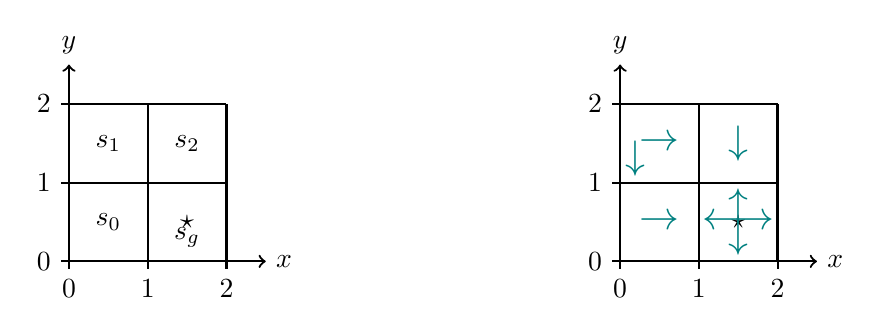
\begin{tikzpicture}
        \tikzstyle{grid}=[draw, thick, fill=gray!10]
        
        % Draw grid
        \draw[grid] (0,0) grid (2,2);
        
        % Add axes
        \draw[thick, ->] (0,0) -- (2.5,0) node[right] {$x$};
        \draw[thick, ->] (0,0) -- (0,2.5) node[above] {$y$};
        
        % Add tick marks and labels
        \foreach \x in {0,1,2} {
            \draw[thick] (\x,0) -- (\x,-0.1) node[below] {$\x$};
        }
        \foreach \y in {0,1,2} {
            \draw[thick] (0,\y) -- (-0.1,\y) node[left] {$\y$};
        }
        
        % Add state labels clockwise from bottom left
        \node at (0.5,0.5) {$s_0$};
        \node at (1.5,0.5) {$\star$};
        \node at (1.5,0.3) {$s_g$};
        \node at (1.5,1.5) {$s_2$};
        \node at (0.5,1.5) {$s_1$};


        % Draw grid
        \draw<2->[grid] (7,0) grid (9,2);
        
        % Add axes
        \draw<2->[thick, ->] (7,0) -- (9.5,0) node[right] {$x$};
        \draw<2->[thick, ->] (7,0) -- (7,2.5) node[above] {$y$};
        
        % Add tick marks and labels
        \draw<2->[thick] (7,0) -- (7,-0.1) node[below] {$0$};
        \draw<2->[thick] (8,0) -- (8,-0.1) node[below] {$1$};
        \draw<2->[thick] (9,0) -- (9,-0.1) node[below] {$2$};
        

        \foreach \y in {0,1,2} {
            \draw<2->[thick] (7,\y) -- (6.9,\y) node[left] {$\y$};
        }
        
        % Add state labels clockwise from bottom left
        \node<2-> at (7.5,0.5) {\Large{\color{teal} $\boldsymbol{\rightarrow}$}};
        \node<2-> at (8.5,0.5) {$\star$};
        \node<2-> at (8.5,0.7) {\Large{\color{teal} $\boldsymbol{\uparrow}$}};
        \node<2-> at (8.5,0.3) {\Large{\color{teal} $\boldsymbol{\downarrow}$}};
        \node<2-> at (8.7,0.5) {\Large{\color{teal} $\boldsymbol{\rightarrow}$}};
        \node<2-> at (8.3,0.5) {\Large{\color{teal} $\boldsymbol{\leftarrow}$}};
        \node<2-> at (8.5,1.5) {\Large{\color{teal} $\boldsymbol{\downarrow}$}};
        \node<2-> at (7.2,1.3) {\Large{\color{teal} $\boldsymbol{\downarrow}$}};
        \node<2-> at (7.5,1.5) {\Large{\color{teal} $\boldsymbol{\rightarrow}$}};
    \end{tikzpicture}}
    \caption*{\onslide<3->{Grid world MDP and optimal actions.}}
    \end{figure}
    \vspace{-0.6cm}
    \begin{figure}
    \centering
    \scalebox{0.85}{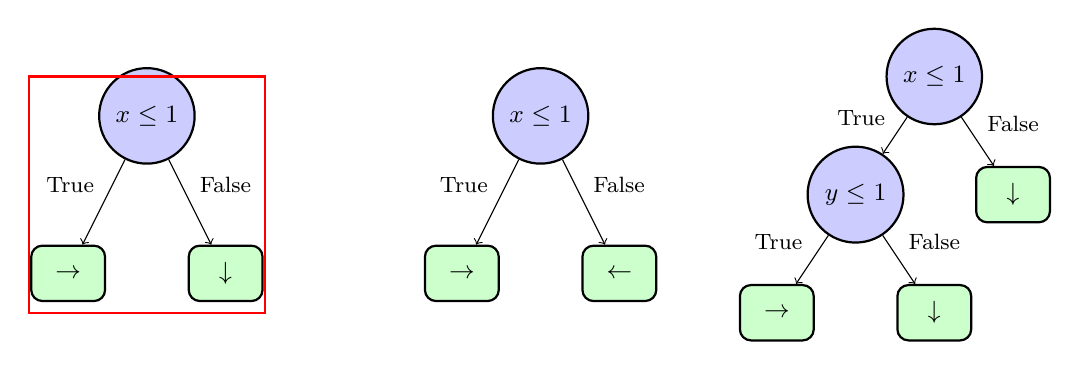
\begin{tikzpicture}[
        decision/.style={circle, draw, thick, fill=blue!20, text width=2.5em, text centered, minimum height=2.5em, font=\small},
        leaf/.style={rectangle, draw, thick, fill=green!20, text width=2em, text centered, rounded corners, minimum height=2em, font=\small},
        edge_label/.style={font=\footnotesize, midway}
    ]
        % Tree 4: if x <= 0.5 move right else move left
        \node<5->[decision] (tree4_root) at (8.5,2) {$x \leq 1$};
        \node<5->[leaf] (tree4_right) at (7.5,0) {$\rightarrow$};
        \node<5->[leaf] (tree4_left) at (9.5,0) {$\leftarrow$};
        \draw<5->[->] (tree4_root) -- (tree4_right) node[edge_label, above left] {True};
        \draw<5->[->] (tree4_root) -- (tree4_left) node[edge_label, above right] {False};
        \tikzstyle{grid}=[draw, thick, fill=gray!10]

        \node<6->[decision] (tree6_root) at (13.5,2.5) {$x \leq 1$};
        \node<6->[decision] (tree6_l) at (12.5,1.) {$y\leq 1$};
        \node<6->[leaf] (tree6_ll) at (11.5,-0.5) {$\rightarrow$};
        \node<6->[leaf] (tree6_lr) at (13.5,-0.5) {$\downarrow$};
        \node<6->[leaf] (tree6_r) at (14.5,1) {$\downarrow$};
        \draw<6->[->] (tree6_root) -- (tree6_l) node[edge_label, above left] {True};
        \draw<6->[->] (tree6_l) -- (tree6_ll) node[edge_label, above left] {True};
        \draw<6->[->] (tree6_l) -- (tree6_lr) node[edge_label, above right] {False};
        \draw<6->[->] (tree6_root) -- (tree6_r) node[edge_label, above right] {False};
        \tikzstyle{grid}=[draw, thick, fill=gray!10]


        % Tree 4: if x <= 0.5 move right else move left
        \node<4->[decision] (tree5_root) at (3.5,2) {$x \leq 1$};
        \node<4->[leaf] (tree5_right) at (2.5,0) {$\rightarrow$};
        \node<4->[leaf] (tree5_left) at (4.5,0) {$\downarrow$};
        \draw<4->[->] (tree5_root) -- (tree5_right) node[edge_label, above left] {True};
        \draw<4->[->] (tree5_root) -- (tree5_left) node[edge_label, above right] {False};
        \tikzstyle{grid}=[draw, thick, fill=gray!10]

        \draw<7->[thick, red] (2, -0.5) rectangle (5, 2.5);


    \end{tikzpicture}}
    \caption*{\onslide<7->{Decision tree policies with different interpretability-performance trade-offs.}}
    \end{figure}
\end{frame}


% \begin{frame}{Grid world MDP and decision tree policies: indirect approach}
% \only<2-3>{\begin{figure}
%     \only<2-3>{\begin{subfigure}{0.65\textwidth}
%     \centering
%     \includegraphics[trim={0 0 15.5cm 0},clip,width=0.9\textwidth]{../images/images_part1/base_mdp.pdf}
%     \caption*{Sample complexity curve of Q-learning over 100 random seeds.}\label{fig:ql-il}
%     \end{subfigure}}
%     \only<3>{\begin{subfigure}{0.24\textwidth}
%     \begin{tikzpicture}
%         \tikzstyle{grid}=[draw, thick, fill=gray!10]
%         % Draw grid
%         \draw[grid] (7,0) grid (9,2);
    
%         % Adds
%         \draw[thick, ->] (7,0) -- (9.5,0) node[right] {$x$};
%         \draw[thick, ->] (7,0) -- (7,2.5) node[above] {$y$};
    
%         % Addk marks and labels
%         \draw[thick] (7,0) -- (7,-0.1) node[below] {$0$};
%         \draw[thick] (8,0) -- (8,-0.1) node[below] {$1$};
%         \draw[thick] (9,0) -- (9,-0.1) node[below] {$2$};
    
%         \foreach \y in {0,1,2} {
%             \draw[thick] (7,\y) -- (6.9,\y) node[left] {$\y$};
%         }
        
%         % Addte labels clockwise from bottom left
%         \node at (7.5,0.6) {\Large{\color{blue} $\boldsymbol{\rightarrow}$}};
%         \node at (7.5,0.4) {\Large{\color{orange} $\boldsymbol{\rightarrow}$}};
%         \node at (8.5,0.5) {$\star$};
%         \node at (8.5,0.3) {\Large{\color{blue} $\boldsymbol{\downarrow}$}};
%         \node at (8.3,0.5) {\Large{\color{orange} $\boldsymbol{\leftarrow}$}};
%         \node at (8.4,1.5) {\Large{\color{orange} $\boldsymbol{\downarrow}$}};
%         \node at (8.6,1.5) {\Large{\color{blue} $\boldsymbol{\downarrow}$}};
%         \node at (7.5,1.6) {\Large{\color{blue} $\boldsymbol{\rightarrow}$}};
%         \node at (7.5,1.4) {\Large{\color{orange} $\boldsymbol{\rightarrow}$}};

%     \end{tikzpicture}
%     \caption*{Expert policies.}
% \end{subfigure}}
% \end{figure}}
% \only<4>{\begin{figure}
%     \centering
%     \includegraphics[width=1\textwidth]{../images/images_part1/base_mdp.pdf}
%     \caption*{Sample complexity curve of Q-learning over 100 random seeds and performance of indirect interpretable methods when imitating the greedy policy with a tree at different Q-learning stages.}\label{fig:ql-il}
% \end{figure}}
% \end{frame}

% \begin{frame}{Direct approach to interpretable SDM}
%     \textit{Q: Can we use reinforcement learning to directly optimize trade-offs of performance and interpretability in SDM?}\\
%     \vspace{1cm}
%     \textbf{A: direct reinforcement leargning is hard because it involves partial observability.}
% \end{frame}

\begin{frame}{Iterative bounding Markov decision processes~\parencite{topin2021iterative}}
\begin{figure}
\centering
\only<1-8>{
    \scalebox{0.7}{
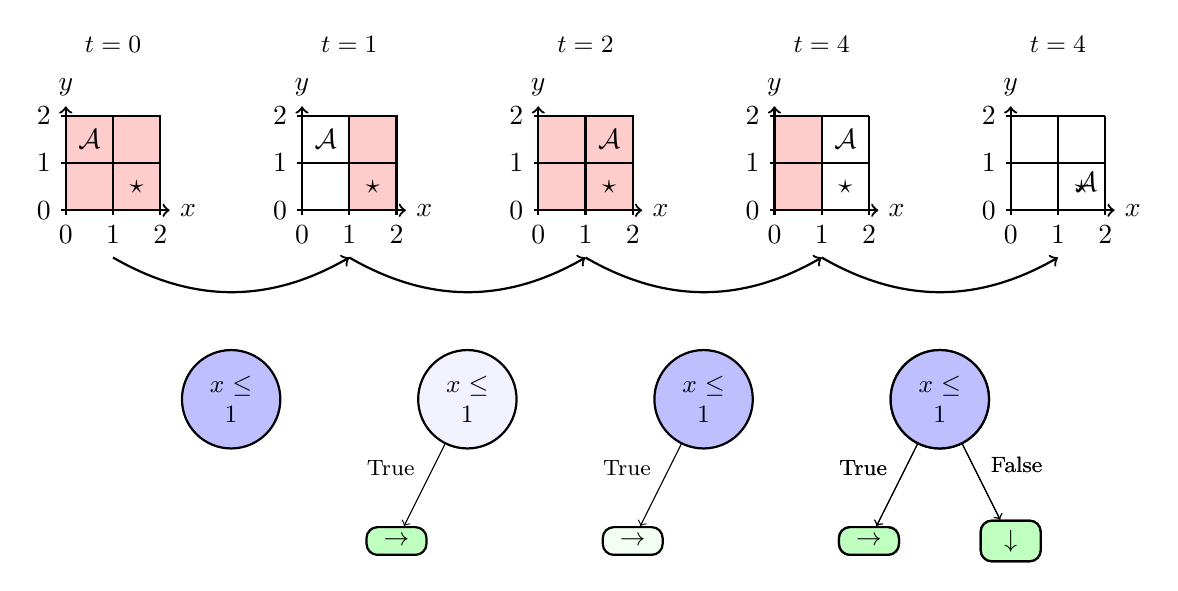
\begin{tikzpicture}[scale=0.6]
    % Define styles
    \tikzstyle{grid}=[draw, thick, fill=gray!10]
    \tikzstyle{rectangle}=[draw, thick, fill=red!20]
    
    % Row 1: IBMDP States (s, o)
    % t=0: Initial state
    \node at (2,7.5) {\small $t=0$};

    \draw<2->[rectangle] (1,4) rectangle (3,6);
    \draw[grid] (1,4) grid (3,6);
    % Add axes
    \draw[thick, ->] (1,4) -- (3.2,4) node[right] {$x$};
    \draw[thick, ->] (1,4) -- (1,6.2) node[above] {$y$};
    \foreach \x in {0,1,2} {
        \draw[thick] (\x+1,4) -- (\x+1,3.9) node[below] {$\x$};
    }
    \foreach \y in {0,1,2} {
        \draw[thick] (1,\y+4) -- (0.9,\y+4) node[left] {$\y$};
    }
    \node at (2.5, 4.5) {$\star$};
    \node<1> at (1.5, 5.5) {$\mathcal{A}$};
    
    % Curved arrow from t=0 to t=1
    \draw<3->[thick, ->] (2,3) to[bend right=30] node[midway, below] {} (7,3);

    % % t=1: After AIG x≤0.5
    \node<3-> at (7,7.5) {\small $t=1$};

    \draw<3->[rectangle] (7,4) rectangle (8,6);
    \draw<3->[grid] (6,4) grid (8,6);
    % Add axes
    \draw<3->[thick, ->] (6,4) -- (8.2,4) node[right] {$x$};
    \draw<3->[thick, ->] (6,4) -- (6,6.2) node[above] {$y$};
    \foreach \x in {0,1,2} {
        \draw<3->[thick] (\x+6,4) -- (\x+6,3.9) node[below] {$\x$};
    }
    \foreach \y in {0,1,2} {
        \draw<3->[thick] (6,\y+4) -- (5.9,\y+4) node[left] {$\y$};
    }
    \node<3-> at (7.5, 4.5) {$\star$};
    \node<3-> at (6.5, 5.5) {$\mathcal{A}$};



    % Curved arrow from t=1 to t=2
    \draw<4->[thick, ->] (7,3) to[bend right=30] node[midway, below] {}(12,3);

    \node<4-> at (12,7.5) {\small $t=2$};
    
    \draw<5->[rectangle] (11,4) rectangle (13,6);
    \draw<4->[grid] (11,4) grid (13,6);
    % Add axes
    \draw<4->[thick, ->] (11,4) -- (13.2,4) node[right] {$x$};
    \draw<4->[thick, ->] (11,4) -- (11,6.2) node[above] {$y$};
    \foreach \x in {0,1,2} {
        \draw<4->[thick] (\x+11,4) -- (\x+11,3.9) node[below] {$\x$};
    }
    \foreach \y in {0,1,2} {
        \draw<4->[thick] (11,\y+4) -- (10.9,\y+4) node[left] {$\y$};
    }
    \node<4-> at (12.5, 4.5) {$\star$};
    \node<4> at (12.5, 5.5) {$\mathcal{A}$};

    
    % Curved arrow from t=2 to t=4
    \draw<6->[thick, ->] (12,3) to[bend right=30] node[midway, below] {} (17,3);
    
    \node<6-> at (17,7.5) {\small $t=4$};

    \draw<6->[rectangle] (16,4) rectangle (17,6);
    \draw<6->[grid] (16,4) grid (18,6);
    % Add axes
    \draw<6->[thick, ->] (16,4) -- (18.2,4) node[right] {$x$};
    \draw<6->[thick, ->] (16,4) -- (16,6.2) node[above] {$y$};
    \foreach \x in {0,1,2} {
        \draw<6->[thick] (\x+16,4) -- (\x+16,3.9) node[below] {$\x$};
    }
    \foreach \y in {0,1,2} {
        \draw<6->[thick] (16,\y+4) -- (15.9,\y+4) node[left] {$\y$};
    }
    \node<6-> at (17.5, 4.5) {$\star$};
    \node<6-> at (17.5, 5.5) {$\mathcal{A}$};

    
    \draw<7->[thick, ->] (17,3) to[bend right=30] node[midway, below] {} (22,3);
    
    % % \node[circle, draw, thick, fill=blue!25, text width=2em, text centered, minimum height=1.5em, font=\small] (tree4_root) at (14.5,0) {$x \leq 1$};
    % % \node[rectangle, draw, thick, fill=green!5, text width=1.5em, text centered, rounded corners, minimum height=1em, font=\small] (tree4_right) at (13,-3) {$\rightarrow$};
    % % \node[rectangle, draw, thick, fill=green!5, text width=1.5em, text centered, rounded corners, minimum height=1em, font=\small] (tree4_left) at (16,-3) {$\downarrow$};
    % % \draw[->] (tree4_root) -- (tree4_right) node[font=\footnotesize, midway, above left] {True};
    % % \draw[->] (tree4_root) -- (tree4_left) node[font=\footnotesize, midway, above right] {False};


    \node<7-> at (22,7.5) {\small $t=4$};
 
    % \draw[rectangle] (21,4) rectangle (23,6);
    \draw<7->[grid] (21,4) grid (23,6);
    % % Add axes
    \draw<7->[thick, ->] (21,4) -- (23.2,4) node[right] {$x$};
    \draw<7->[thick, ->] (21,4) -- (21,6.2) node[above] {$y$};
    \foreach \x in {0,1,2} {
        \draw<7->[thick] (\x+21,4) -- (\x+21,3.9) node[below] {$\x$};
    }
    \foreach \y in {0,1,2} {
        \draw<7->[thick] (21,\y+4) -- (20.9,\y+4) node[left] {$\y$};
    }
    \node<7-> at (22.5, 4.5) {$\star$};
    \node<7-> at (22.6, 4.6) {$\mathcal{A}$};


    % \node[circle, draw, thick, fill=blue!5, text width=2em, text centered, minimum height=1.5em, font=\small] (tree4_root) at (19.5,0) {$x \leq 1$};
    % \node[rectangle, draw, thick, fill=green!5, text width=1.5em, text centered, rounded corners, minimum height=1em, font=\small] (tree4_right) at (18,-3) {$\rightarrow$};
    % \node[rectangle, draw, thick, fill=green!25, text width=1.5em, text centered, rounded corners, minimum height=1em, font=\small] (tree4_left) at (21,-3) {$\downarrow$};
    % \draw[->] (tree4_root) -- (tree4_right) node[font=\footnotesize, midway, above left] {True};
    % \draw[->] (tree4_root) -- (tree4_left) node[font=\footnotesize, midway, above right] {False};
    \node<7>[circle, draw, thick, fill=blue!5, text width=2em, text centered, minimum height=1.5em, font=\small] (tree4_root) at (19.5,0) {$x \leq 1$};
    \node<7>[rectangle, draw, thick, fill=green!5, text width=1.5em, text centered, rounded corners, minimum height=1em, font=\small] (tree4_right) at (18,-3) {$\rightarrow$};
    \node<7>[rectangle, draw, thick, fill=green!25, text width=1.5em, text centered, rounded corners, minimum height=1em, font=\small] (tree4_left) at (21,-3) {$\downarrow$};
    \draw<7>[->] (tree4_root) -- (tree4_right) node[font=\footnotesize, midway, above left] {True};
    \draw<7>[->] (tree4_root) -- (tree4_left) node[font=\footnotesize, midway, above right] {False};

    \node<8->[circle, draw, thick, fill=blue!25, text width=2em, text centered, minimum height=1.5em, font=\small] (tree4_root) at (19.5,0) {$x \leq 1$};
    \node<8->[rectangle, draw, thick, fill=green!25, text width=1.5em, text centered, rounded corners, minimum height=1em, font=\small] (tree4_right) at (18,-3) {$\rightarrow$};
    \node<8->[rectangle, draw, thick, fill=green!25, text width=1.5em, text centered, rounded corners, minimum height=1em, font=\small] (tree4_left) at (21,-3) {$\downarrow$};
    \draw<8->[->] (tree4_root) -- (tree4_right) node[font=\footnotesize, midway, above left] {True};
    \draw<8->[->] (tree4_root) -- (tree4_left) node[font=\footnotesize, midway, above right] {False};


    \node<6->[circle, draw, thick, fill=blue!25, text width=2em, text centered, minimum height=1.5em, font=\small] (tree4_root) at (14.5,0) {$x \leq 1$};
    \node<6->[rectangle, draw, thick, fill=green!5, text width=1.5em, text centered, rounded corners, minimum height=1em, font=\small] (tree4_right) at (13,-3) {$\rightarrow$};
    % \node<6->[rectangle, draw, thick, fill=green!5, text width=1.5em, text centered, rounded corners, minimum height=1em, font=\small] (tree4_left) at (16,-3) {$\downarrow$};
    \draw<6->[->] (tree4_root) -- (tree4_right) node[font=\footnotesize, midway, above left] {True};
    % \draw<6->[->] (tree4_root) -- (tree4_left) node[font=\footnotesize, midway, above right] {False};

    \node<4->[circle, draw, thick, fill=blue!5, text width=2em, text centered, minimum height=1.5em, font=\small] (tree4_root) at (9.5,0) {$x \leq 1$};
    \node<4->[rectangle, draw, thick, fill=green!25, text width=1.5em, text centered, rounded corners, minimum height=1em, font=\small] (tree4_right) at (8,-3) {$\rightarrow$};
    \draw<4->[->] (tree4_root) -- (tree4_right) node[font=\footnotesize, midway, above left] {True};

    \node<3->[circle, draw, thick, fill=blue!25, text width=2em, text centered, minimum height=1.5em, font=\small] (tree4_root) at (4.5,0) {$x \leq 1$};
    % \node<5>[rectangle, draw, thick, fill=green!5, text width=1.5em, text centered, rounded corners, minimum height=1em, font=\small] (tree4_right) at (3,-3) {$\rightarrow$};
    % \node<5>[rectangle, draw, thick, fill=green!5, text width=1.5em, text centered, rounded corners, minimum height=1em, font=\small] (tree4_left) at (6,-3) {$\downarrow$};
    % \draw<5>[->] (tree4_root) -- (tree4_right) node[font=\footnotesize, midway, above left] {True};
    % \draw<5>[->] (tree4_root) -- (tree4_left) node[font=\footnotesize, midway, above right] {False};

    
\end{tikzpicture}}}
\end{figure}
\only<9->{
\onslide<9->{Given an MDP $\mathcal{M}$ $\langle S, A, R, T \rangle$}\onslide<10->{, an IBMDP is an MDP $$\langle \overbrace{S \times O}^{\text{State space}}, \underbrace{A \cup A_{info}}_{\text{Action space}}, \overbrace{(R, \zeta)}^{\text{Reward function}}, \underbrace{(T_{info}, T)}_{\text{Transitions}}\rangle$$
where:}
\begin{itemize}
    \item<11-> $O$: observations of some state features.
    \item<12-> $A_{info}$: actions that gather informations about some state features.
    \item<13-> $\zeta$: reward for taking $a\in A_{info}$.
    \item<14-> $T_{info}$: transitions following $a\in A_{info}$ that update the partial observation with gathered info.
    \item<15-> \textbf{\warning IBMDP policies $\pi_{po}: O\rightarrow A\cup A_{info}$ are decision tree policies for $\mathcal{M}$.}
\end{itemize}}
\end{frame}

% \begin{frame}{Grid world IBMDP example}
% \begin{figure}
% \centering
% \scalebox{0.7}{
% \begin{tikzpicture}[scale=0.6]
%     % Define styles
%     \tikzstyle{grid}=[draw, thick, fill=gray!10]
%     \tikzstyle{rectangle}=[draw, thick, fill=red!20]
    
%     % Row 1: IBMDP States (s, o)
%     % t=0: Initial state
%     \node<1-> at (2,9.5) {\small $t=0$};
%     \node<1-19> at (2,8.5) {\small $\boldsymbol{s}_t=(0.5, 1.5)$};
%     \node<2-> at (2,7.5) {\small $\boldsymbol{o}_t=(0, 2, 0, 2)$};

%     \draw<2->[rectangle] (1,4) rectangle (3,6);
%     \draw<1->[grid] (1,4) grid (3,6);
%     % Add axes
%     \draw<1->[thick, ->] (1,4) -- (3.2,4) node[right] {$x$};
%     \draw<1->[thick, ->] (1,4) -- (1,6.2) node[above] {$y$};
%     \foreach \x in {0,1,2} {
%         \draw<1->[thick] (\x+1,4) -- (\x+1,3.9) node[below] {$\x$};
%     }
%     \foreach \y in {0,1,2} {
%         \draw<1->[thick] (1,\y+4) -- (0.9,\y+4) node[left] {$\y$};
%     }
%     \node<1-19> at (1.5, 5.5) {$\mathcal{A}$};
%     \node<1-> at (2.5, 4.5) {$\star$};
    
%     % Curved arrow from t=0 to t=1
%     \draw<3->[thick, ->] (2,3) to[bend right=30] node[midway, below] {\small $a_t = \langle x, 1\rangle, r_t = \zeta$} (7,3);

%     % % t=1: After AIG x≤0.5
%     \node<6-> at (7,9.5) {\small $t=1$};
%     \node<6-19> at (7,8.5) {\small $\boldsymbol{s}_t=(0.5, 1.5)$};
%     \node<7-> at (7,7.5) {\small $\boldsymbol{o}_t=(0, 1, 0, 2)$};

%     \draw<7->[rectangle] (6,4) rectangle (7,6);
%     \draw<6->[grid] (6,4) grid (8,6);
%     % Add axes
%     \draw<6->[thick, ->] (6,4) -- (8.2,4) node[right] {$x$};
%     \draw<6->[thick, ->] (6,4) -- (6,6.2) node[above] {$y$};
%     \foreach \x in {0,1,2} {
%         \draw<6->[thick] (\x+6,4) -- (\x+6,3.9) node[below] {$\x$};
%     }
%     \foreach \y in {0,1,2} {
%         \draw<6->[thick] (6,\y+4) -- (5.9,\y+4) node[left] {$\y$};
%     }
%     \node<6-19> at (6.5, 5.5) {$\mathcal{A}$};
%     \node<6-> at (7.5, 4.5) {$\star$};


%     % Curved arrow from t=1 to t=2
%     \draw<8->[thick, ->] (7,3) to[bend right=30] node[midway, below] {\small $a_t = \rightarrow, r_t  = 0$}(12,3);

%     \node<4->[circle, draw, thick, fill=blue!25, text width=2em, text centered, minimum height=1.5em, font=\small] (tree4_root) at (4.5,0) {$x \leq 1$};
%     \node<9-12>[rectangle, draw, thick, fill=green!25, text width=1.5em, text centered, rounded corners, minimum height=1em, font=\small] (tree4_right) at (3,-3) {$\rightarrow$};
%     \node<16->[rectangle, draw, thick, fill=green!25, text width=1.5em, text centered, rounded corners, minimum height=1em, font=\small] (tree4_left) at (6,-3) {$\downarrow$};
%     \draw<9-12>[->] (tree4_root) -- (tree4_right) node[font=\footnotesize, midway, above left] {True};
%     \draw<16->[->] (tree4_root) -- (tree4_left) node[font=\footnotesize, midway, above right] {False};
%     % % \node<13>[circle, draw, thick, fill=blue!5, text width=2em, text centered, minimum height=1.5em, font=\small] (tree4_root) at (4.5,0) {$x \leq 1$};
%     \node<13-17>[rectangle, draw, thick, fill=green!5, text width=1.5em, text centered, rounded corners, minimum height=1em, font=\small] (tree4_right_new) at (3,-3) {$\rightarrow$};
%     \draw<13-17>[->] (tree4_root) -- (tree4_right_new) node[font=\footnotesize, midway, above left] {True};
%     \node<18->[rectangle, draw, thick, fill=green!25, text width=1.5em, text centered, rounded corners, minimum height=1em, font=\small] (tree4_right_new_new) at (3,-3) {$\rightarrow$};
%     \draw<18->[->] (tree4_root) -- (tree4_right_new_new) node[font=\footnotesize, midway, above left] {True};

%     \node<10-> at (12,9.5) {\small $t=2$};
%     \node<10-19> at (12,8.5) {\small $\boldsymbol{s}_t=(1.5, 1.5)$};
%     \node<11-> at (12,7.5) {\small $\boldsymbol{o}_t=(0, 2, 0, 2)$};
    
%     \draw<11->[rectangle] (11,4) rectangle (13,6);
%     \draw<10->[grid] (11,4) grid (13,6);
%     % Add axes
%     \draw<10->[thick, ->] (11,4) -- (13.2,4) node[right] {$x$};
%     \draw<10->[thick, ->] (11,4) -- (11,6.2) node[above] {$y$};
%     \foreach \x in {0,1,2} {
%         \draw<10->[thick] (\x+11,4) -- (\x+11,3.9) node[below] {$\x$};
%     }
%     \foreach \y in {0,1,2} {
%         \draw<10->[thick] (11,\y+4) -- (10.9,\y+4) node[left] {$\y$};
%     }
%     \node<10-19> at (12.5, 5.5) {$\mathcal{A}$};
%     \node<10-> at (12.5, 4.5) {$\star$};
    
%     % Curved arrow from t=2 to t=4
%     \draw<12->[thick, ->] (12,3) to[bend right=30] node[midway, below] {\small $a_t = \langle x, 1 \rangle, r_t = \zeta$} (17,3);

%     % \node<13->[circle, draw, thick, fill=blue!25, text width=2em, text centered, minimum height=1.5em, font=\small] (tree4_root) at (9.5,0) {$x \leq 1$};
%     % \node[rectangle, draw, thick, fill=green!25, text width=1.5em, text centered, rounded corners, minimum height=1em, font=\small] (tree4_right) at (8,-3) {$\rightarrow$};
%     % \node[rectangle, draw, thick, fill=green!5, text width=1.5em, text centered, rounded corners, minimum height=1em, font=\small] (tree4_left) at (11,-3) {$\downarrow$};
%     % \draw[->] (tree4_root) -- (tree4_right) node[font=\footnotesize, midway, above left] {True};
%     % \draw[->] (tree4_root) -- (tree4_left) node[font=\footnotesize, midway, above right] {False};

    
%     \node<14-> at (17,9.5) {\small $t=4$};
%     \node<14-19> at (17,8.5) {\small $\boldsymbol{s}_t=(1.5, 1.5)$};
%     \node<14-> at (17,7.5) {\small $\boldsymbol{o}_t=(1, 2, 0, 2)$};

%     \draw<14->[rectangle] (17,4) rectangle (18,6);
%     \draw<14->[grid] (16,4) grid (18,6);
%     % Add axes
%     \draw<14->[thick, ->] (16,4) -- (18.2,4) node[right] {$x$};
%     \draw<14->[thick, ->] (16,4) -- (16,6.2) node[above] {$y$};
%     \foreach \x in {0,1,2} {
%         \draw<14->[thick] (\x+16,4) -- (\x+16,3.9) node[below] {$\x$};
%     }
%     \foreach \y in {0,1,2} {
%         \draw<14->[thick] (16,\y+4) -- (15.9,\y+4) node[left] {$\y$};
%     }
%     \node<14-19> at (17.5, 5.5) {$\mathcal{A}$};
%     \node<14-> at (17.5, 4.5) {$\star$};
    
%     \draw<15->[thick, ->] (17,3) to[bend right=30] node[midway, below] {\small $a_t = \downarrow, r_t = 0$} (22,3);
    
%     % % \node[circle, draw, thick, fill=blue!25, text width=2em, text centered, minimum height=1.5em, font=\small] (tree4_root) at (14.5,0) {$x \leq 1$};
%     % % \node[rectangle, draw, thick, fill=green!5, text width=1.5em, text centered, rounded corners, minimum height=1em, font=\small] (tree4_right) at (13,-3) {$\rightarrow$};
%     % % \node[rectangle, draw, thick, fill=green!5, text width=1.5em, text centered, rounded corners, minimum height=1em, font=\small] (tree4_left) at (16,-3) {$\downarrow$};
%     % % \draw[->] (tree4_root) -- (tree4_right) node[font=\footnotesize, midway, above left] {True};
%     % % \draw[->] (tree4_root) -- (tree4_left) node[font=\footnotesize, midway, above right] {False};


%     \node<17-> at (22,9.5) {\small $t=5$};
%     \node<17-19> at (22,8.5) {\small $\boldsymbol{s}_t=(1.5, 0.5)$};
%     \node<17-> at (22,7.5) {\small $\boldsymbol{o}_t=(0, 2, 0, 2)$};
 
%     \draw<17->[rectangle] (21,4) rectangle (23,6);
%     \draw<17->[grid] (21,4) grid (23,6);
%     % % Add axes
%     \draw<17->[thick, ->] (21,4) -- (23.2,4) node[right] {$x$};
%     \draw<17->[thick, ->] (21,4) -- (21,6.2) node[above] {$y$};
%     \foreach \x in {0,1,2} {
%         \draw<17->[thick] (\x+21,4) -- (\x+21,3.9) node[below] {$\x$};
%     }
%     \foreach \y in {0,1,2} {
%         \draw<17->[thick] (21,\y+4) -- (20.9,\y+4) node[left] {$\y$};
%     }
%     \node<17-19> at (22.5, 4.5) {$\mathcal{A}$};
%     \node<17-> at (22.5, 4.5) {$\star$};

%     % \node[circle, draw, thick, fill=blue!5, text width=2em, text centered, minimum height=1.5em, font=\small] (tree4_root) at (19.5,0) {$x \leq 1$};
%     % \node[rectangle, draw, thick, fill=green!5, text width=1.5em, text centered, rounded corners, minimum height=1em, font=\small] (tree4_right) at (18,-3) {$\rightarrow$};
%     % \node[rectangle, draw, thick, fill=green!25, text width=1.5em, text centered, rounded corners, minimum height=1em, font=\small] (tree4_left) at (21,-3) {$\downarrow$};
%     % \draw[->] (tree4_root) -- (tree4_right) node[font=\footnotesize, midway, above left] {True};
%     % \draw[->] (tree4_root) -- (tree4_left) node[font=\footnotesize, midway, above right] {False};

    
% \end{tikzpicture}}
% \end{figure}
% \begin{itemize}
%     \item<19-20>{Topin et. al. show that only certain policies correspond to decision trees.}
% \end{itemize}
% \end{frame}
\setbeamercovered{transparent}
\begin{frame}{RL for memoryless policies in POMDPs}
    \onslide<1->{\begin{alertblock}{RL for memoryless policies}
        \begin{itemize}
        \item<2-> Finding the best deterministic and memoryless policy in a POMDP is NP-hard \textcolor{purple}{\small \parencite{littman1}}!
        \item<3-> The best memoryless policy can be stochastic \textcolor{purple}{\small \parencite{learning-pomdp}}.
        \item<4-> Value-based RL converges to sub-optimal solutions.
    \end{itemize}}
    \end{alertblock}
    \onslide<5->{\begin{block}{Asymmetric RL {\small \parencite{pinto}}}
        \begin{itemize}
            \item<6-> Value-based $\rightarrow$ learns $Q(o, a)$ with TD targets $U(s, a)$  \textcolor{purple}{\small \parencite{baisero-dqn}}.
            \item<7-> Actor-critic $\rightarrow$ policy gradient on $\pi(o, a)$ using a critic $V(s)$ \textcolor{purple}{\small \parencite{baisero-ppo}}.
            \item<8-> Supposed to work better for our problem \textcolor{purple}{\small \parencite{justif-asym}}.
        \end{itemize}
    \end{block}}
\end{frame}

\begin{frame}{Result: RL cannot retrieve optimal depth-1 trees for the grid world MDP}
\begin{figure}
    \centering
    \includegraphics[width=1\textwidth]{tree_distributions.pdf}
    \caption*{Distributions of tree policies learned with (asymmetric) RL algorithms as a function of the interpretability reward $\zeta$.}
\end{figure}
\end{frame}

\begin{frame}{Direct RL of decision trees for classification tasks does not involve partial observability}
\begin{figure}
    \centering
    \begin{tikzpicture}[
        decision/.style={circle, draw, thick, fill=blue!20, text width=2.5em, text centered, minimum height=2.5em, font=\small},
        leaf/.style={rectangle, draw, thick, fill=green!20, text width=2em, text centered, rounded corners, minimum height=2em, font=\small},
        edge_label/.style={font=\footnotesize, midway}
    ]
        % Tree 4: if x <= 0.5 move right else move left
        \node[decision] (tree4_root) at (8,2) {$x \leq 1$};
        \node[rectangle, draw, thick, fill=green!40, text width=2em, text centered, rounded corners, minimum height=2em, font=\small] (tree4_right) at (7,0) {};
        \node[rectangle, draw, thick, fill=red!40, text width=2em, text centered, rounded corners, minimum height=2em, font=\small] (tree4_left) at (9,0);
        \draw[->] (tree4_root) -- (tree4_right) node[edge_label, above left] {True};
        \draw[->] (tree4_root) -- (tree4_left) node[edge_label, above right] {False};
        \tikzstyle{grid}=[draw, thick, fill=gray!10]
        
        % Draw grid
        \draw[fill=green!40] (0, 0) rectangle (1,2);
        \draw[fill=red!40] (1, 0) rectangle (2,2);

        \draw[grid] (0,0) grid (2,2);
        
        % Add axes
        \draw[thick, ->] (0,0) -- (2.5,0) node[right] {$x$};
        \draw[thick, ->] (0,0) -- (0,2.5) node[above] {$y$};
        
        % Add tick marks and labels
        \foreach \x in {0,1,2} {
            \draw[thick] (\x,0) -- (\x,-0.1) node[below] {$\x$};
        }
        \foreach \y in {0,1,2} {
            \draw[thick] (0,\y) -- (-0.1,\y) node[left] {$\y$};
        }

        \node at (0.5,0.5) {$\boldsymbol{s}_0$};
        \node at (1.5,0.5) {$\boldsymbol{s}_g$};
        \node at (1.5,1.5) {$\boldsymbol{s}_2$};
        \node at (0.5,1.5) {$\boldsymbol{s}_1$};
    \end{tikzpicture}
    \caption*{Classification MDP and the unique optimal depth-1 tree.}
\end{figure}
\only<2>{\textbf{\textcolor{teal}{Partial observations are sufficient statistics of the full states in IBMDPs for classification tasks.}}}
\end{frame}

\begin{frame}{Result: RL can retrieve optimal depth-1 trees for the toy classification MDP}
\begin{figure}
    \centering
    \includegraphics[width=1\textwidth]{tree_distributions_merged.pdf}
    \caption*{Distributions of tree policies learned with various RL algorithms.
    }
\end{figure}
\end{frame}


% \begin{frame}{Experimental result: for SDM problems $\Leftrightarrow$ classification problems, RL can consistently retrieve optimal depth-1 decision tree policies}
% \begin{figure}
%     \centering
%     \includegraphics[width=1\textwidth]{../images/images_part1/tree_distributions_classif.pdf}
%     \caption*{Each colored dot is the number of final learned trees with a specific structure for a given $\zeta$. Those results makes sense because we can show that IBMDPs for classification tasks don't have a partial observability component.}\label{fig:tree-distrib-classif-poibmdp}
% \end{figure}
% \end{frame}
\setbeamercovered{transparent}
\begin{frame}{Perspectives for direct RL of decision tree policies.}
    \begin{itemize}
        \pause
        \item It seems that directly learning decision tree trading off interpretability and performances in MDPs can be difficult to achieve because of \textcolor{red}{\textbf{partial observability}}.
        \pause
        \item Should we focus on indirect approaches? Hybrid approaches {\small \textcolor{purple}{\parencite{parbhoo}}}?
        \pause
        \item Fixing the policy tree structure a priori (parametric trees, {\small \textcolor{purple}{\parencite{sympol}}})?
        % \pause
        % \item Can other policies (programs, oblique trees, algebraic expressions\dots) be directly optimized with RL in IBMDPs?
        % \pause
        % \item Design algorithms that learn deterministic memoryless policies in POMDPs {\small \textcolor{purple}{\parencite{lambrechts2025informed,justif-asym}}}?
    \end{itemize}
    \pause
    \begin{exampleblock}{RL can train good decision trees for classification MDPs}
    \pause
    \textit{Q: Can we leverage SDM to design new decision tree induction algorithms for classification/regression?}
    \end{exampleblock}
\end{frame}

\begin{frame}{Decision trees in supervised learning}
\begin{itemize}
    \pause
    \item $N$ data points $\{\boldsymbol{x}_i,y_i\}$. Each $\boldsymbol{x}_i$ is described by $p$ features and has a label $y_i \in {\mathcal Y}$. 
    We want to find a tree of depth at most $D$, $T\in\mathcal{T}_D$ that minimizes:
    \begin{align*}
        \mathcal{L}_{\alpha}(T) = \frac{1}{N}\overset{N}{\underset{i=1}{\sum}}{\ell}(y_i, T(x_i)) + \alpha C(T)
    \end{align*}
    \pause
    \item Trees \textbf{interpretable} and \textbf{competitive with neural nets} {\small \textcolor{purple}{\parencite{grinsztajn2022tree}}}.
    \pause
    \item Greedy algorithms \textcolor{red}{\textbf{sub-optimal accuracy}}, but \textcolor{teal}{$\boldsymbol{O(2^D)}$} operations {\small \textcolor{purple}{\parencite{breiman1984classification}}} .
    \pause
    \item Optimal algorithms, \textcolor{teal}{\textbf{optimal accuracy}}, but \textcolor{red}{$\boldsymbol{O((2Np)^D)}$} operations (NP-hard) {\small \textcolor{purple}{\parencite{oct}}}.
    \pause
    \item In between optimal and greedy?
\end{itemize}
\end{frame}

\begin{frame}{Decision tree induction as solving MDPs}
\pause
\begin{block}{Intuition}
    The induction of a decision tree is made of a sequence of decisions: at each node, we must decide whether it is better to split (a subset of) the training data, or %assign a class label and 
    to create a leaf node.
\end{block}
\begin{itemize}
    \pause
    \item S: data subsets.
    \pause
    \item A: test or leaf nodes that can be added to the tree.
    \pause
    \item R: interpretability term $-\alpha$ and misclassifications.
    \pause
    \item T: node traversals.
\end{itemize}
\pause
\begin{proposition}[Objective Equivalence]
Let $\pi$ be a deterministic policy of the MDP. 
Then $J_\alpha(\pi) = -{\mathcal L}_\alpha(E(\pi, s_0))$ where $E$ is an algorithm that extracts a decision tree from $\pi$ \textcolor{purple}{\small \parencite{topin2021iterative}}.
\end{proposition}
\end{frame}
\setbeamercovered{invisible}

% \begin{frame}{Objective Leftrightarrowalence}
% \begin{block}{Objective Equivalence}\label{prop:Leftrightarrow}
% Let $\pi$ be a deterministic policy of the MDP and $\pi^*$ be an optimal deterministic policy. 
% Then $J_\alpha(\pi) = -{\mathcal L}_\alpha(E(\pi, s_0))$ and $T^* = E(\pi^*, s_0)$ where $T^*$ is a tree that optimizes Eq.~\ref{eq:suplearning}.
% \end{block}
% \begin{alertblock}{Interpretation}
% We can learn a decision tree that maximizes accuracy by finding an MDP policy that maximizes rewards (this can be done easily with DP).
% \end{alertblock}
% \end{frame}
\setbeamercovered{transparent}
\begin{frame}{Controlling the time complexity of decision tree induction}

\begin{itemize}
    \pause
    \item Greedy algorithms consider only one candidate action in each state which is the test that minimizes some impurity criterion \\
    \pause
    $\rightarrow$ \textcolor{teal}{\textbf{MDP state space size is} $\boldsymbol{O(2^D)}$}.
    \pause
    \item Optimal algorithms consider all possible actions in each state \\
    \pause
    $\rightarrow$ \textcolor{red}{\textbf{MDP state space size is} $\boldsymbol{O((2Np)^D)}$}.
    \pause
    \item \textbf{Dynamic Programming Decision Trees (DPDT)}: Let's choose candidate actions adaptively \\
    \pause
    $\rightarrow$ for each MDP state consider $B$ actions: \textcolor{blue}{\textbf{state space size is} $\boldsymbol{O((2B)^D)}$}.
    \\
    \pause
    $\rightarrow$ solve the MDP exactly with DP.
\end{itemize}
\pause
\vspace{0.4cm}
{\Large \textbf{\textcolor{blue}{How to choose the $B$ candidate actions/splits?}}}
\pause
\\
Top-B greedy splits \textcolor{purple}{\small \parencite{topk}}, quantiles, random\dots
\end{frame}

\begin{frame}{Practical implemenataion of DPDT}
\begin{figure}
    \centering
    \includegraphics[width=0.8\linewidth]{../images/figures/schematic_cart_node_select.pdf}
    \pause
    \caption*{We can use greedy trees nodes as candidate actions.}
\end{figure}
\end{frame}
% \begin{frame}{DPDT trees can be strictly better than greedy trees}
%     \begin{figure}
%         \centering
%         \includegraphics[width=1\textwidth]{Présentation sans titre (16).png}
%     \end{figure}
% \end{frame}
% \begin{frame}{DPDT trees can be strictly better than greedy trees}
%     \begin{figure}
%         \centering
%         \includegraphics[width=1\textwidth]{Présentation sans titre (17).png}
%     \end{figure}
% \end{frame}
% \begin{frame}{DPDT trees can be strictly better than greedy trees}
%     \begin{figure}
%         \centering
%         \includegraphics[width=1\textwidth]{Présentation sans titre (18).png}
%     \end{figure}
% \end{frame}
\setbeamercovered{invisible}
\begin{frame}{Fast like greedy trees, accurate like optimal trees}
    \begin{figure}
    \centering
    \includegraphics[width=0.85\textwidth]{mirror_accuracy_vs_cost.pdf}
    \end{figure}
    \only<1>{Train accuracies against cost for detph-3 trees.}
    \begin{itemize}
        \item<2-> DPDT trees can are not worse than greedy trees.
        \item<3-> DPDT trees can be strictly better than greedy trees.
        \item<4-> CART generates more diverse splits than Top B for DPDT. 
    \end{itemize}
\end{frame}

\begin{frame}{Large scale evaluation of DPDT trees generalization {\small \parencite{grinsztajn2022tree}}}
    \only<2>{\begin{figure}
    \centering
        \includegraphics[width=0.6\textwidth]{../images/figures/tab_bench/random_search_classif_numerical_depth5.pdf}
        \caption*{DPDT depth-5 trees vs. other detph-5 trees}
    \end{figure}}
    \only<3>{\begin{figure}
         \centering
         \includegraphics[width=0.6\textwidth]{../images/figures/tab_bench/random_search_classif_categorical_boosting_w_weak.pdf}
         \caption*{Boosted DPDT vs. Boosted CART}
     \end{figure}}
     \only<4>{\begin{figure}
         \centering
         \includegraphics[width=0.6\textwidth]{../images/figures/tab_bench/random_search_classif_numerical_boosting_all_notgb.pdf}
         \caption*{Boosted DPDT vs. other classifiers}
     \end{figure}}
\end{frame}



%-------------LONNNNNNNNNNNNNNG


\begin{frame}{Perspectives}
    \begin{itemize}
        \pause
        \item New SOTA decision tree induction with dynamic programming in MDPs.
        \pause
        \item What about using DPDT for indirect decision tree policy learning for SDM?
        \pause
        \item What performances could we reach with an industry-grade implementation of XGboost+DPDT?
    \end{itemize}
    \pause
    \begin{exampleblock}{Let us take a step back}
        \textit{Q: Are decision trees really the most interpretable model?}\\
    \end{exampleblock}
\end{frame}

\begin{frame}{How to measure policy interpretability?}
\onslide<1->{\begin{alertblock}{Challenges {\small \parencite{rigourous}}}
\begin{itemize}
    \item<2-> No unified formal definition of policy interpretability.
    \item<3-> Measuring requires humans.
    \item<11-> Different hardwares (CPUs vs GPUs).
    \item<12-> Different implementations (matrix operations vs fully sequentially) {\small \textcolor{purple}{\parencite{insight}}}
\end{itemize}
\end{alertblock}}

\onslide<4->{\begin{exampleblock}{The notion of \textit{simulatability} {\small \parencite{lipton}}}
\begin{itemize}
    \item<5-> {
    \only<5-8>{Interpretability $\simeq$ time for a human to compute the same.}
    \only<9->{Interpretability $\simeq$ \textbf{\textcolor{blue}{runtime in seconds?}}}
    }
    \item<6-> {
        \only<6-9>{Interpretability $\simeq$ how much effort for a human to read through the entire policy.}
        \only<10->{Interpretability $\simeq$ \textbf{\textcolor{blue}{size in bytes?}}}
    }
    \item<7-> Less parameters mean more interpretability {\small \textcolor{purple}{\parencite{study-0}}}.
    \item<8-> Time to formally verify a policy decreases with interpretability {\small \textcolor{purple}{\parencite{lens-complexity}}}.
\end{itemize}
\end{exampleblock}}
\end{frame}

% \begin{frame}{A methodology to measure policy interpretability without humans}
% \pause
% \begin{block}{Simulatability {\small \parencite{lipton}}}
% \begin{enumerate}
%     \pause
%     \item How long it takes for human to make the same computations given an input $\simeq$ policy inference time.
%     \pause
%     \item How much effort it would take a human to read through the entire policy once $\simeq$ policy size in memory.
% \end{enumerate}
% \end{block}
% \pause
% \begin{alertblock}{Not that simple in practice {\small \textcolor{purple}{\parencite{insight}}}}
% \begin{itemize}
%     \pause
%     \item Different hardwares (CPUs vs GPUs).
%     \pause
%     \item Different implementations (matrix operations vs fully sequentially) $\dots$
% \end{itemize}
% \end{alertblock}
% \end{frame}

% \begin{frame}{Empirical validation}
% \begin{enumerate}
%     \pause
%     \item Is policy unfolding necessary?
%     \pause
%     \item What kind of results we can obtain using our proposed methodology?
% \end{enumerate}
% \pause
% \begin{block}{Setup}
% We imitate $\sim40000$ expert policies from \texttt{stable-baselines3} using various policy classes/nb parameters on various environments.
% \end{block}
% \end{frame}


% \begin{frame}{Empirical validation: obtaining $\sim40000$ policies from different classes}
% \begin{table}[ht]
% \{-0.3cm}
% \centering
% \footnotesize
% \begin{tabular}{lll}
% \hline
% \textbf{Policy Class} & \textbf{Parameters} & \textbf{Training algo.} \\
% \hline
% Linear policies & Determined by state-action dimensions & Linear/logistic Reg. \\
% Decision trees & \{4, 8, 16, 64, 128\} nodes & CART \\
% Oblique decision trees & \{4, 8, 16, 64, 128\} nodes & CART \\
% Relu neural networks & \{(2 ,2), (4, 4), (8, 8), (16, 16)\} weights & SGD \\
% \hline
% \end{tabular}
% \caption*{Summary of policy classes parameters and supervised learning algorithms to fit experts.}
% \end{table}
% \end{frame}

% \begin{frame}{Empirical validation: obtaining $\sim40000$ policies from different classes}

% \begin{table}[ht]
% \hspace{-0.48cm}
%   \centering
%   \footnotesize
%   \begin{tabular}{lll}
%   \hline
%   \textbf{Classic} & \textbf{MuJoCo} & \textbf{OCAtari}\\
%   \hline
%   CartPole (4, 2, \textbf{490}) & Swimmer (8, 2, \textbf{300}) & Breakout (452, 4, \textbf{30})\\
%   LunarLander (8, 4, \textbf{200}) & Walker2d (17, 6, \textbf{2000}) & Pong (20, 6, \textbf{14})\\
%   //    Continuous (8, 2, \textbf{200}) & HalfCheetah (17, 6, \textbf{3000}) & SpaceInvaders (188, 6, \textbf{680})\\
%   BipedalWalker (24, 4, \textbf{250}) & Hopper (11, 3, \textbf{2000}) & Seaquest (180, 18, \textbf{2000})\\
%   MountainCar (2, 3, \textbf{90}) & \\
%   //    Continuous (2, 1, \textbf{-110}) & \\
%   Acrobot (6, 3, \textbf{-100}) & \\
%   Pendulum (3, 1, \textbf{-400}) & \\
%   \hline
%   \end{tabular}
%   \caption*{Summary of considered environments (dimensions of states and number or dimensions of actions, \textbf{performance thresholds to solve}). OCAtari is an object-centric version of Atari.}
%   \end{table}

% \end{frame}

\begin{frame}[fragile]{We propose policy unfolding}
\begin{tcolorbox}
\begin{lstlisting}[language=Python]
# Small ReLU MLP for Pendulum
def play(x):
    h_layer_0_0 = 1.68 * x[0] + -0.69 * x[1] + -0.74 * x[2] + -1.40
    h_layer_0_0 = max(0.0, h_layer_0_0)
    h_layer_0_1 = 0.20 * x[0] + 0.29 * x[1] + -0.021 * x[2] + 1.25
    h_layer_0_1 = max(0.0, h_layer_0_1)
    h_layer_0_2 = 0.33 * x[0] + -0.57 * x[1] + 0.47 * x[2] + 1.94
    h_layer_0_2 = max(0.0, h_layer_0_2)
    h_layer_0_3 = 1.39 * x[0] + 0.94 * x[1] + 0.50 * x[2] + -1.13
    h_layer_0_3 = max(0.0, h_layer_0_3)
    h_layer_1_0 = 1.16 * h_layer_0_0 + -1.59 * h_layer_0_1 + 0.95 * h_layer_0_2 + -1.22 * h_layer_0_3 + -0.54
    h_layer_1_0 = max(0.0, h_layer_1_0)
    h_layer_1_1 = -0.55 * h_layer_0_0 + 1.13 * h_layer_0_1 + -0.58 * h_layer_0_2 + -0.72 * h_layer_0_3 + 1.56
    h_layer_1_1 = max(0.0, h_layer_1_1)
    h_layer_1_2 = 1.10 * h_layer_0_0 + -1.01 * h_layer_0_1 + 0.96 * h_layer_0_2 + -2.84 * h_layer_0_3 + -0.02
    h_layer_1_2 = max(0.0, h_layer_1_2)
    h_layer_1_3 = 0.27 * h_layer_0_0 + 0.44 * h_layer_0_1 + 0.39 * h_layer_0_2 + 0.15 * h_layer_0_3 + -1.24
    h_layer_1_3 = max(0.0, h_layer_1_3)
    h_layer_2_0 = -2.80 * h_layer_1_0 + -0.60 * h_layer_1_1 + 3.07 * h_layer_1_2 + -1.63 * h_layer_1_3 + -0.36
    y_0 = h_layer_2_0

    return [y_0]
\end{lstlisting}
\end{tcolorbox}
\end{frame}

\begin{frame}{Is time/size of unfolded policies a good proxy?}
\onslide<1->{\begin{block}{Setup}
We imitate $\sim40000$ expert policies from \texttt{stable-baselines3} using various policy classes/nb parameters on various environments.
\end{block}}
\onslide<2->{\begin{figure}
    \centering
    \includegraphics[width=1\linewidth]{../images/images_part3/tree_sizes_memory_ppo_ci_ablation.pdf}
    \caption*{Aggregated policies interpretability on classic control environments}
\end{figure}}
\end{frame}



\setbeamercovered{transparent}
\begin{frame}{Perspectives}
\begin{itemize}
    \pause
    \item Beliefs such as "trees are more interpretable than neural networks" should be used with caution.
    % \pause
    % \item Tree-like policy classes can have good inductive bias (e.g. Atari).
    \pause
    \item What about floating points precision?
    \pause
    \item What about the cost of basic operations ($\times$ vs. $+$ vs. $\geq$)?
\end{itemize}
\end{frame}

\begin{frame}{Conclusion: interpretable SDM is a difficult research topic}
    \begin{itemize}
        \pause
        \item \textbf{Technical challenges:} \textcolor{red}{\textbf{Learning interpretable policies for SDM involves partial observability.}}
        \\
        \pause
        $\rightarrow$ Focus on indirect approaches and/or on POMDP research first?
        \\
        \pause
        $\rightarrow$ \textbf{\textcolor{teal}{Created opportunities for new decision tree algos for classif/regression.}}
        \item \textbf{Fundamental challenges:} \textcolor{red}{\textbf{No concensus on interpretability definition}}. 
        \\
        \pause
        $\rightarrow$ Keep exploring benchmarks for policy interpretability.
        \\
        $\rightarrow$ Discuss with the community (InterpPol workshop).
    \end{itemize}
    \pause
    \begin{block}{My hope}
        Motivate interpretability by finding a real-world problem where interpretability is \textit{really} necessary {\small \textcolor{purple}{\parencite{festor}}}.
    \end{block}
\end{frame}

\begin{frame}{Broader perspectives}
    \begin{itemize}
        \pause
        \item \textbf{\textcolor{purple}{Deep learning:}} Can we design deep learning layers that take datasets and output candidate splits?
        \pause
        \item \textbf{\textcolor{blue}{Combinatorial optimization:}} Can we formulate other combinatorial/NP-hard problems as MDPs and design other DPDT-like algorithms?
        \pause
        \item \textbf{\textcolor{orange}{Human-computer interaction:}} Can we do large scale human study of the $\sim$40K programs interpertability?
    \end{itemize}
\end{frame}
\setbeamercovered{invisible}
\printbibliography
\appendix


\begin{frame}[noframenumbering]{Result: for similar problems, RL struggles more when there is partial observability}
\only<1>{\begin{figure}
    \centering
    \includegraphics[trim={3cm 15.2cm 20cm 1cm},clip,width=0.3\textwidth]{barplot_with_std.pdf}
\end{figure}}
\only<2->{\begin{figure}
    \centering
    \includegraphics[width=0.7\textwidth]{barplot_with_std.pdf}
\end{figure}}
\vspace{-0.4cm}
{\small Success rates over thousands of RL runs with varying hyperparameters when learning different policies in the same IBMDP\footnote{\tiny We also observed similar results on classic controls and variants of the grid world MDP.}.
}
\end{frame}


\begin{frame}[noframenumbering]{Decision tree induction as solving MDPs}
\only<1>{\begin{figure}
    \centering
    \includegraphics[width=1\linewidth]{schema AAAI (5).png}
    \caption*{Example of decision tree induction as an MDP.}
\end{figure}}
\only<2>{\begin{figure}
    \centering
    \includegraphics[width=1\linewidth]{schema AAAI (1).png}
    \caption*{Example of decision tree induction as an MDP.}
\end{figure}}
\only<3>{\begin{figure}
    \centering
    \includegraphics[width=1\linewidth]{schema AAAI (2).png}
    \caption*{Example of decision tree induction as an MDP.}
\end{figure}
}
\only<4>{\begin{figure}
    \centering
    \includegraphics[width=1\linewidth]{schema AAAI (3).png}
    \caption*{Example of decision tree induction as an MDP.}
\end{figure}
}
\only<5>{\begin{figure}
    \centering
    \includegraphics[width=1\linewidth]{schema AAAI (4).png}
    \caption*{Example of decision tree induction as an MDP.}
\end{figure}
}
\end{frame}

\begin{frame}[noframenumbering]{Fast like greedy trees, accurate like optimal trees}
    \begin{figure}
        \centering
        \includegraphics[width=1\linewidth]{../images/figures/patho_bounds_comparison_checkers.pdf}
        \caption*{Comparison of greedy, optimal, and DPDT  depth-2 trees on the checkersboard dataset.}
    \end{figure}
\end{frame}

\begin{frame}[noframenumbering]{Fast like greedy trees, accurate like optimal trees}
\begin{table}
    \centering
    \tiny
    \caption*{Comparison of accuracies and operations for depth-3 trees.}
    \scalebox{0.8}{\begin{tabular}{l|cccccc|cccccc}
    \toprule
    & \multicolumn{6}{c|}{\textbf{Accuracy}} & \multicolumn{6}{c}{\textbf{Operations}} \\
    \midrule
    \textbf{Dataset} & Opt & Greedy & \multicolumn{4}{c}{DPDT} & Opt & Greedy & \multicolumn{4}{c}{DPDT} \\
    &  &  &
    CART^{-} & CART^{+} &
    TopB^{-} & TopB^{+} &
     &  &
    CART^{-} & CART^{+} &
    TopB^{-} & TopB^{+} \\
    \midrule
    room    & \textbf{0.992} & 0.968 & \color{blue}0.991 & \textbf{0.992} & 0.990 & \textbf{0.992} & $10^6$       & 15 & 286 & 16100 & 111 & 16100 \\
    bean    & \textbf{0.871} & 0.777 & 0.812 & \color{blue}0.853 & 0.804 & 0.841 & $5\cdot10^6$   & 15 & 295 & 25900 & 112 & 16800 \\
    eeg     & \textbf{0.708} & 0.666 & 0.689 & \color{blue}0.706 & 0.684 & 0.699 & $2\cdot10^6$   & 13 & 289 & 26000 & 95  & 11000 \\
    avila   & \textbf{0.585} & 0.532 & \color{blue}0.574 & \textbf{0.585} & 0.563 & 0.572 & $3\cdot10^7$   & 9  & 268 & 24700 & 60  & 38900 \\
    magic   & \textbf{0.831} & 0.801 & 0.822 & \color{blue}0.828 & 0.807 & 0.816 & $6\cdot10^6$   & 15 & 298 & 28000 & 70  & 4190  \\
    htru    & \textbf{0.981} & 0.979 & 0.979 & \color{blue}0.980 & 0.979 & \color{blue}0.980 & $6\cdot10^7$   & 15 & 295 & 25300 & 55  & 2180  \\
    occup.  & \textbf{0.994} & 0.989 & 0.991 & \textbf{0.994} & 0.990 & \color{blue}0.992 & $7\cdot10^5$   & 13 & 280 & 16300 & 33  & 510   \\
    skin    & \textbf{0.969} & \color{blue}0.966 & \color{blue}0.966 & \color{blue}0.966 & \color{blue}0.966 & \color{blue}0.966 & $7\cdot10^4$   & 15 & 301 & 23300 & 20  & 126   \\
    fault   & \textbf{0.682} & 0.553 & 0.672 & \color{blue}0.674 & 0.672 & 0.673 & $9\cdot10^8$   & 13 & 295 & 24200 & 111 & 16800 \\
    segment & \textbf{0.887} & 0.574 & 0.812 & \color{blue}0.879 & 0.786 & 0.825 & $2\cdot10^6$   & 7  & 220 & 16300 & 68  & 11400 \\
    page    & \textbf{0.971} & 0.964 & \color{blue}0.970 & \color{blue}0.970 & 0.964 & 0.965 & $10^7$        & 15 & 298 & 22400 & 701 & 4050  \\
    bidding & \textbf{0.993} & 0.981 & \color{blue}0.985 & \textbf{0.993} & 0.985 & \textbf{0.993} & $3\cdot10^5$   & 13 & 256 & 9360  & 58  & 2700  \\
    raisin  & \textbf{0.894} & 0.869 & 0.879 & \color{blue}0.886 & 0.875 & 0.883 & $4\cdot10^6$   & 15 & 295 & 20900 & 48  & 1440  \\
    rice    & \textbf{0.938} & 0.933 & 0.934 & \color{blue}0.937 & 0.933 & 0.936 & $2\cdot10^7$   & 15 & 298 & 25500 & 49  & 1470  \\
    wilt    & \textbf{0.996} & 0.993 & 0.994 & \color{blue}0.995 & 0.994 & 0.994 & $3\cdot10^5$   & 13 & 274 & 11300 & 33  & 465   \\
    bank    & \textbf{0.983} & 0.933 & 0.971 & \color{blue}0.980 & 0.951 & 0.974 & $6\cdot10^4$   & 13 & 271 & 7990  & 26  & 256   \\
    \bottomrule
    \end{tabular}}
\end{table}
\end{frame}

\begin{frame}[noframenumbering]{CART generates more diverse splits than Top B}
    \only<1>{\begin{figure}
        \centering
        \includegraphics[width=0.95\textwidth]{../images/figures/splits_tsne_topknaive.pdf}
    \end{figure}}
    \only<2>{\begin{figure}
        \centering
        \includegraphics[width=0.95\textwidth]{../images/figures/splits_tsne_dpdt.pdf}
    \end{figure}}
\end{frame}

\setbeamercovered{transparent}
\begin{frame}[noframenumbering]{Why generating candidate splits with CART?}
    \pause
    \begin{theorem}[DPDT trees are not worse than greedy trees]
    \pause
    The greedy tree is always a solution of the MDPs we solve. Because we solve the MDPs exactly with DP, if the greedy tree is the best solution, DPDT will find it.
    \end{theorem}
    \pause
    \begin{theorem}[DPDT trees can be strictly better than greedy trees]
    \pause
    There exist a depth budget $D$ and a dataset for which DPDT trees are strictly better than greedy trees.\footnote{cf. checkersboard dataset.}
    \end{theorem}
\end{frame}
\setbeamercovered{invisible}

\begin{frame}[noframenumbering]{DPDT trees can be strictly better than greedy trees}
    \only<1>{\begin{figure}
        \centering
        \includegraphics[width=1\textwidth]{Présentation sans titre.png}
    \end{figure}}
    \only<2>{\begin{figure}
        \centering
        \includegraphics[width=1\textwidth]{Présentation sans titre (1).png}
    \end{figure}}
    \only<3>{\begin{figure}
        \centering
        \includegraphics[width=1\textwidth]{Présentation sans titre (2).png}
    \end{figure}}
    \only<4>{\begin{figure}
        \centering
        \includegraphics[width=1\textwidth]{Présentation sans titre (3).png}
    \end{figure}}
    \only<5>{\begin{figure}
        \centering
        \includegraphics[width=1\textwidth]{Présentation sans titre (4).png}
    \end{figure}}
    \only<6>{\begin{figure}
        \centering
        \includegraphics[width=1\textwidth]{Présentation sans titre (5).png}
    \end{figure}}
    \only<7>{\begin{figure}
        \centering
        \includegraphics[width=1\textwidth]{Présentation sans titre (6).png}
    \end{figure}}
    \only<8>{\begin{figure}
        \centering
        \includegraphics[width=1\textwidth]{Présentation sans titre (7).png}
    \end{figure}}
    \only<9>{\begin{figure}
        \centering
        \includegraphics[width=1\textwidth]{Présentation sans titre (8).png}
    \end{figure}}
    \only<10>{\begin{figure}
        \centering
        \includegraphics[width=1\textwidth]{Présentation sans titre (9).png}
    \end{figure}}
    \only<11>{\begin{figure}
        \centering
        \includegraphics[width=1\textwidth]{Présentation sans titre (10).png}
    \end{figure}}
    \only<12>{\begin{figure}
        \centering
        \includegraphics[width=1\textwidth]{Présentation sans titre (13).png}
    \end{figure}}
\end{frame}

\begin{frame}[noframenumbering]{Result: verification time does scale with step inference time}
    \begin{figure}[ht]
    \centering
    \includegraphics[width=1\linewidth]{../images/images_part3/verification_tradeoff.pdf}
    \caption*{Verification time as a function of policy interpretability. Top row, interpretability is measured with step inference times. Bottom row, the interpretability is measured with policy size.}
    \label{fig:trade-off-verif}
\end{figure}
\end{frame}

\begin{frame}[noframenumbering]{Result: there is no dominating policy class for all environments}
\begin{figure}
    \centering
    \includegraphics[trim={1.4cm 0 0 0},clip,width=1\textwidth]{../images/images_part3/trade_off_select_combine_one_plot.pdf}
    \caption*{Interpretability-Performance trade-offs. Top row, interpretability is measured with step inference times. Bottom row, the interpretability is measured with policy size.}
\end{figure}
\end{frame}


\begin{frame}[noframenumbering,fragile]{We propose policy unfolding}
\begin{minipage}{0.48\textwidth}
\begin{tcolorbox}
\begin{lstlisting}[language=Python]
# Decision tree for Mountain Car
def play(x):
    if x[1] <= -0.2597:
        if x[1] <= -0.6378:
            return 0
        else:
            if x[0] <= -1.0021:
                return 2
            else:
                return 0
    else:
        if x[1] <= -0.0508:
            if x[0] <= 0.2979:
                if x[0] <= 0.0453:
                    return 2
                else:
                    if x[1] <= -0.2156:
                        return 0
                    else:
                        return 2
            else:
                return 0
        else:
            return 2
\end{lstlisting}
\end{tcolorbox}
\end{minipage}
\hfill
\begin{minipage}{0.5\textwidth}
\begin{tcolorbox}
\begin{lstlisting}[language=Python]
# Small ReLU MLP for Pendulum
def play(x):
    h_layer_0_0 = 1.238*x[0]+0.971*x[1]
                  +0.430*x[2]+0.933
    h_layer_0_0 = max(0, h_layer_0_0)
    h_layer_0_1 = -1.221*x[0]+1.001
                  *x[1]-0.423*x[2]
                  +0.475
    h_layer_0_1 = max(0, h_layer_0_1)
    h_layer_1_0 = -0.109*h_layer_0_0
                  -0.377*h_layer_0_1
                  +1.694
    h_layer_1_0 = max(0, h_layer_1_0)
    h_layer_1_1 = -3.024*h_layer_0_0
                  -1.421*h_layer_0_1
                  +1.530
    h_layer_1_1 = max(0, h_layer_1_1)

    h_layer_2_0 = -1.790*h_layer_1_0
                  +2.840*h_layer_1_1
                  +0.658
    y_0 = h_layer_2_0
    return [y_0]
\end{lstlisting}
\end{tcolorbox}
\end{minipage}
\end{frame}
\end{document}